% CAPÍTULO 2 — FUNDAMENTAÇÃO TEÓRICO -----------------------------------------------------------------------

\chapter{Fundamentação Teórica}
\label{cap:referencial}

Este capítulo reúne os fundamentos que sustentam o trabalho. Começa caracterizando o mercado de trabalho em TI no Brasil e as bases de dados oficiais que o registram; em seguida, apresenta os conceitos de engenharia de dados e a arquitetura adotada, as tecnologias de armazenamento e consulta e as ferramentas de visualização; por fim, descreve os modelos de séries temporais usados na previsão e encerra com uma discussão dos trabalhos relacionados.

\section{O Mercado de Trabalho em TI no Brasil}

Nas últimas décadas, o setor de Tecnologia da Informação (TI) no Brasil cresceu sem grandes interrupções. Por trás desse movimento estão a transformação digital de empresas e órgãos públicos, a expansão do comércio eletrônico e os modelos de negócio centrados em plataformas digitais. De acordo com o Relatório Setorial 2024 da BRASSCOM, o macrossetor de Tecnologia, Informação e Comunicação (TIC) já responde por 6,5\% do Produto Interno Bruto (PIB) brasileiro, com produção setorial de R\$~762,4 bilhões e crescimento médio de 8,4\% ao ano nos três anos anteriores \cite{Brasscom2024}. Em 2024, o setor reunia cerca de 2,1 milhões de empregos formais, o equivalente a 3,8\% de todos os vínculos celetistas do país.

Uma pesquisa da Federação do Comércio de Bens, Serviços e Turismo do Estado de São Paulo, baseada nos microdados da RAIS, mostrou que as profissões ligadas à tecnologia cresceram 95\% entre 2012 e 2022 e que, em alguns casos, como o de engenheiro de sistemas operacionais, a alta passou de 740\% no mesmo período \cite{Fecomercio2024}. Esse ritmo, porém, não vem sendo acompanhado pela oferta de mão de obra qualificada. Entre 2019 e 2024, o mercado precisou de 665.403 profissionais de TI, enquanto apenas 464.569 se formaram no período, um déficit estrutural de cerca de 30\%
\cite{Brasscom2025}.

A pandemia de COVID-19 acelerou esse cenário. A partir de 2020, empresas de todos os portes adotaram em escala maior ferramentas de colaboração remota, \textit{cloud computing} e automação, o que ampliou a procura por profissionais de TI justamente no momento em que o restante do mercado formal sofria forte contração \cite{CAGED2024}. Há também um efeito geográfico relevante. O emprego em TI segue concentrado no Sudeste, sobretudo em São Paulo, mas vem se espalhando pelo país desde 2020. Em 2024, a Região Norte registrou o maior crescimento percentual de contratações no setor TIC (7,4\%), movimento associado à difusão do trabalho remoto, que tornou estados fora do eixo Sul-Sudeste mais atrativos para a contratação de profissionais de TI \cite{Brasscom2024}.

Estudar essas dinâmicas em profundidade exige fontes com cobertura nacional, série histórica longa e granularidade por ocupação. Entre as bases disponíveis no Brasil, RAIS e CAGED são as únicas que atendem a esses três requisitos ao mesmo tempo.

\section{Bases de Dados Governamentais: RAIS e CAGED}

Esta seção descreve as duas fontes oficiais que alimentam o trabalho, a RAIS e o CAGED, além das tabelas auxiliares necessárias para interpretar seus códigos. Para cada base, destacam-se a origem, a estrutura dos arquivos, a evolução do formato ao longo do tempo e as implicações para o tratamento dos dados.

\subsection{RAIS: Relação Anual de Informações Sociais}

A RAIS é um registro administrativo criado pelo Decreto n.º 76.900/1975. O preenchimento é anual e obrigatório para todos os estabelecimentos com empregados formais, sejam celetistas, estatutários, avulsos ou outros. A cada ano-base, são declarados os vínculos ativos em 31 de dezembro e os encerrados ao longo do ano, com informações como cargo (CBO), salário de dezembro, carga horária, grau de instrução, gênero, raça/cor, tempo de emprego, município e CNAE do estabelecimento \cite{RAIS2024}.

Os arquivos distribuídos pelo MTE são compostos apenas por códigos numéricos: não há cabeçalhos, e os valores textuais ficam por conta de tabelas de tradução externas. Cada campo ocupa uma posição fixa de bytes definida em arquivos de \textit{layout} que acompanham cada base. O tamanho varia muito entre estados e anos: a RAIS do Acre em 2007 tem cerca de 39~MB, enquanto a de São Paulo em 2022 passa de 10~GB, o que reflete tanto o tamanho do mercado quanto a cobertura crescente ao longo do tempo. Essa natureza puramente numérica deixa os arquivos ilegíveis sem os \textit{layouts} e os dicionários de CBO, CNAE e municípios, mas em compensação ajuda bastante na compressão em Parquet: colunas de inteiros repetidos, como códigos de município, são codificadas com dicionário e comprimidas com ZSTD com eficiência muito maior do que em dados textuais.

Neste trabalho, a RAIS é a principal fonte para descrever o estoque de empregos formais em TI, ou seja, o total de vínculos ativos por ocupação, estado e setor em cada 31 de dezembro. Sua série, disponível desde 1985 e com boa qualidade a partir dos anos 2000, viabiliza análises de longo prazo da evolução do setor.

A RAIS tem uma limitação importante: captura só o mercado formal. Ela não enxerga trabalhadores por conta própria, microempreendedores individuais (MEI) nem profissionais autônomos sem CNPJ, segmentos que têm crescido bastante no setor de TI \cite{IPEA2023}. Como é uma declaração anual, também não dá para observar sazonalidade dentro do mesmo ano, lacuna que o CAGED ajuda a preencher.


\subsection{CAGED: Cadastro Geral de Empregados e Desempregados}

\subsubsection{Formato Antigo do CAGED (2007--2019)}

O CAGED foi criado pela Lei n.º 4.923/1965 como instrumento de controle das admissões e demissões de empregados regidos pela Consolidação das Leis do Trabalho (CLT). No formato vigente até dezembro de 2019, os empregadores declaravam mensalmente cada movimentação ocorrida no mês, e o MTE disponibilizava os dados em um único arquivo de largura fixa (\textit{fixed-width}) por competência \cite{CAGED2024}.

Cada registro traz cerca de 40 campos com informações sobre o trabalhador (idade, gênero, grau de instrução, salário mensal, CBO, tempo de emprego) e o estabelecimento (CNAE, município, porte, subsetor IBGE). Há ainda campos de regionalização fina para alguns municípios, como bairros de São Paulo, Rio de Janeiro e Fortaleza, além de distritos, mesorregiões e microrregiões. Cada linha representa uma movimentação, e um campo indica se ela é uma admissão ou um desligamento; o saldo líquido do mês é a diferença entre admissões e desligamentos.

\subsubsection{Novo CAGED (2020--2025)}

Em janeiro de 2020, o CAGED foi reformulado pela Portaria n.º 1.127/2019 e passou a fazer parte do sistema eSocial, recebendo o nome de \textit{Cadastro Geral de Empregados e Desempregados Estoque} (CAGEDEST). Quatro pontos mudam em relação ao formato antigo \cite{CAGED2024}:

\begin{itemize}
    \item \textbf{Formato}: de um único arquivo de largura fixa para CSV compactado (\texttt{.7z}), com separador ponto e vírgula;
    \item \textbf{Tipos de arquivo}: o que antes era um arquivo único passa a ser dividido em quatro tipos: \textbf{MOV} (declarações regulares, 31 campos) e \textbf{FOR} (fora do prazo, mesmo esquema do MOV) constituem o fluxo principal; \textbf{EXC} (exclusões, 33 campos, com colunas adicionais de competência de exclusão e indicador de cancelamento) registra as retificações; e \textbf{AJUSTES} (correções retroativas integradas ao eSocial, 45 campos) cobre reclassificações retroativas de competências que remontam a 2010;
    \item \textbf{Colunas}: esquema reformulado com 31 campos nos tipos MOV e FOR, incluindo variáveis novas como horas contratuais, indicador de trabalho intermitente e parcial, código de categoria do trabalhador e valor do salário fixo; os campos de
    regionalização granular do formato antigo (bairros, distritos, mesorregiões) foram
    suprimidos;
    \item \textbf{Codificação}: os tipos MOV\slash{}FOR\slash{}EXC são distribuídos em Latin-1, mantendo a mesma codificação do CAGED antigo; o tipo AJUSTES utiliza UTF-8.  Essa convivência de duas codificações no mesmo período exige tratamento explícito no  \textit{parser}, sob risco de gerar registros com caracteres corrompidos.
\end{itemize}

Com a divisão em vários arquivos, o saldo de cada competência deixa de sair de uma única fonte: passa a ser preciso somar as movimentações de MOV e FOR e descontar as de EXC para chegar ao número correto.

Essa diferença de formato, esquema e codificação entre os dois períodos é um dos maiores desafios técnicos do trabalho e demanda estratégias específicas de harmonização no \textit{pipeline}.

\subsection{Tabelas Auxiliares e CBO}

A CBO é o documento oficial que descreve, agrupa e organiza as ocupações do mercado de trabalho brasileiro. Ela serve de base para preencher os campos de cargo na RAIS e no CAGED \cite{CBO2024}. A classificação é hierárquica e segue quatro níveis:

\begin{itemize}
    \item \textbf{Grande Grupo} (1 dígito): nível mais agregado, organiza as ocupações por natureza do trabalho (e.g., Grande Grupo~2 para profissionais das ciências e das artes; Grande Grupo~3 para técnicos de nível médio);
    \item \textbf{Subgrupo Principal} (2 dígitos) e \textbf{Subgrupo} (3 dígitos): níveis intermediários de agregação;
    \item \textbf{Família Ocupacional} (4 dígitos): unidade básica de classificação, agrupando ocupações com tarefas similares;
    \item \textbf{Ocupação} (6 dígitos): nível mais específico, descreve cargos individuais.
\end{itemize}

A \autoref{fig:cbo-hierarquia} mostra essa estrutura na prática, usando uma ocupação de TI como exemplo: o código de 6 dígitos pertence, ao mesmo tempo, a todos os níveis hierárquicos mais agregados.

\begin{figure}[htbp]
    \centering
    \caption{Hierarquia da CBO com exemplo do setor de TI}
    \label{fig:cbo-hierarquia}
    \begin{tikzpicture}[
        every node/.style={font=\footnotesize},
        nivel/.style={rectangle, rounded corners=2pt, draw=black!60, thick,
                      minimum height=12mm, align=center, inner sep=4pt},
        rotulo/.style={font=\scriptsize\itshape, anchor=west},
        seta/.style={-{Stealth[length=2mm]}, thick, black!60}
    ]
        % Niveis (esquerda para direita)
        \node[nivel, fill=blue!10,   minimum width=2.6cm] (n1) at (0,0)
            {\textbf{2} \\ Grande Grupo};
        \node[nivel, fill=orange!15, minimum width=2.6cm, right=8mm of n1] (n2)
            {\textbf{21} \\ Subgrupo Principal};
        \node[nivel, fill=green!12,  minimum width=2.6cm, right=8mm of n2] (n3)
            {\textbf{2124} \\ Família Ocupacional};
        \node[nivel, fill=purple!12, minimum width=2.8cm, right=8mm of n3] (n4)
            {\textbf{212405} \\ Ocupação};

        % Setas
        \draw[seta] (n1) -- (n2);
        \draw[seta] (n2) -- (n3);
        \draw[seta] (n3) -- (n4);

        % Descricoes dos niveis
        \node[align=center, font=\scriptsize, below=2mm of n1, text width=2.8cm]
            {Profissionais das ciências e das artes};
        \node[align=center, font=\scriptsize, below=2mm of n2, text width=2.8cm]
            {Profissionais das ciências exatas e da engenharia};
        \node[align=center, font=\scriptsize, below=2mm of n3, text width=2.8cm]
            {Analistas de Tecnologia da Informação};
        \node[align=center, font=\scriptsize, below=2mm of n4, text width=3.0cm]
            {Analista de Sistemas (Suporte)};

        % Indicacao dos digitos
        \node[font=\scriptsize\itshape, above=2mm of n1] {1 dígito};
        \node[font=\scriptsize\itshape, above=2mm of n2] {2 dígitos};
        \node[font=\scriptsize\itshape, above=2mm of n3] {4 dígitos};
        \node[font=\scriptsize\itshape, above=2mm of n4] {6 dígitos};

    \end{tikzpicture}
    \\[4pt]
    Fonte: Autoria própria, baseado em \citeonline{CBO2024}.
\end{figure}

A delimitação do setor de TI neste trabalho acontece no nível de família ocupacional (4 dígitos). Esse nível reúne ocupações tecnicamente equivalentes em um único código e é o que se manteve mais estável ao longo dos 18 anos da série.

\subsection{CNAE e Tabela de Municípios}

A CBO classifica o que o trabalhador faz, mas não diz em que tipo de empresa ele atua. Esse papel cabe à CNAE, que organiza os estabelecimentos pelo setor econômico em que operam. A CNAE é mantida pelo IBGE e estruturada de forma hierárquica em cinco níveis, do mais agregado (Seção, com letras de A a U) ao mais específico (Subclasse, com 7 dígitos numéricos) \cite{CNAE2024}.

No contexto deste trabalho, o CNAE permite distinguir quem atua em empresas de tecnologia propriamente ditas (Divisão 62, ``Atividades dos serviços de tecnologia da informação'') de quem ocupa funções de TI em outros setores, como bancos, indústria ou comércio. É o cruzamento entre CBO (ocupação) e CNAE (setor) que viabiliza perguntas como ``quantos analistas de sistemas trabalham em bancos \textit{versus} em empresas de \textit{software}?'', revelando o quanto o setor extrapola seu próprio recorte econômico.

Por fim, a tabela de municípios do IBGE é utilizada para traduzir os códigos numéricos de município presentes na RAIS e no CAGED em nomes legíveis e, sobretudo, para agrupar os vínculos por unidade federativa. Sem essa tradução, qualquer análise regional ficaria inviável. As três tabelas (CBO, CNAE e municípios) são distribuídas pelo MTE no mesmo servidor FTP das bases principais.

Usadas juntas, RAIS e CAGED dão uma visão que nenhuma das duas oferece sozinha. A RAIS funciona como uma fotografia anual dos vínculos ativos em 31 de dezembro, útil para acompanhar o nível absoluto de emprego por ocupação, estado e setor ao longo dos anos. Já o CAGED é o filme mensal das admissões e desligamentos, mostrando sazonalidade, dinâmica intra-anual e rupturas pontuais, como a contração brusca de março de 2020. Uma dá o nível; a outra mostra como ele se move ao longo do ano. É a combinação das duas que fecha o quadro do emprego formal.

\section{Engenharia de Dados e Arquitetura Medalhão}

\subsection{\textit{Data Lake} e as Camadas Bronze, Silver e Gold}

O \textit{data lake} surgiu como alternativa ao \textit{data warehouse} tradicional para lidar com grandes volumes de dados heterogêneos \cite{Reis2022}. A distinção principal entre os dois está em \textit{quando} o esquema é fixado: o \textit{data warehouse} obriga a modelar tudo num esquema rígido antes de gravar (\textit{schema on write}), ao passo que o \textit{data lake} guarda o dado bruto e só o transforma na hora da consulta ou de forma incremental (\textit{schema on read}). Para projetos como este, em que os dados de origem chegam em formatos heterogêneos e as regras de transformação podem mudar ao longo do tempo, essa flexibilidade faz bastante diferença.

A Arquitetura Medalhão (\textit{Medallion Architecture}), popularizada pelo ecossistema Databricks, organiza o \textit{data lake} em camadas sucessivas de qualidade crescente. Segundo a \citeonline{MicrosoftMedallion2024}, as camadas Bronze (bruto), Silver (validado) e Gold (enriquecido) descrevem a qualidade crescente dos dados ao longo do fluxo. Neste trabalho, elas se organizam da seguinte forma:

\begin{itemize}
    \item \textbf{Bronze}: armazena os dados brutos exatamente como recebidos da fonte, sem nenhuma transformação. Essa camada é imutável e serve como fonte de verdade para reprocessamento. No contexto desta pesquisa, contém os arquivos originais da RAIS e do CAGED baixados do FTP do MTE;

    \item \textbf{Silver}: contém os dados após limpeza, padronização, enriquecimento e filtragem. Os dados brutos são parseados, os códigos são traduzidos por dicionários externos e os registros são filtrados ao domínio de interesse (setor de TI). O resultado é armazenado em formato otimizado para análise (Parquet);

    \item \textbf{Gold}: contém os dados agregados e modelados para consumo direto por ferramentas analíticas, \textit{dashboards} e modelos de aprendizado de máquina. As agregações pré-computadas reduzem o tempo de resposta das consultas no \textit{dashboard} e fornecem as séries temporais prontas para modelagem preditiva.
\end{itemize}

Separar os dados em camadas traz rastreabilidade (\textit{lineage}): se algo dá errado em uma camada, basta corrigir e reprocessar as seguintes a partir da Bronze, sem precisar baixar de novo os arquivos do MTE.

\subsection{Apache Parquet e Compressão Colunar}

O Apache Parquet é um formato de armazenamento colunar criado originalmente para o ecossistema Hadoop e mantido pela Apache Software Foundation \cite{ApacheParquet2024}. Nos formatos orientados a linha, como CSV ou JSON, todos os campos de um mesmo registro ficam juntos no disco. O Parquet inverte essa lógica e agrupa os valores de cada coluna em sequência. A \autoref{fig:parquet-vs-csv} compara as duas abordagens usando uma tabela simples, com quatro colunas (Ano, UF, CBO e Saldo) e três registros.

\begin{figure}[htbp]
    \centering
    \caption{Comparação entre armazenamento orientado a linha (CSV) e a coluna (Parquet)}
    \label{fig:parquet-vs-csv}
    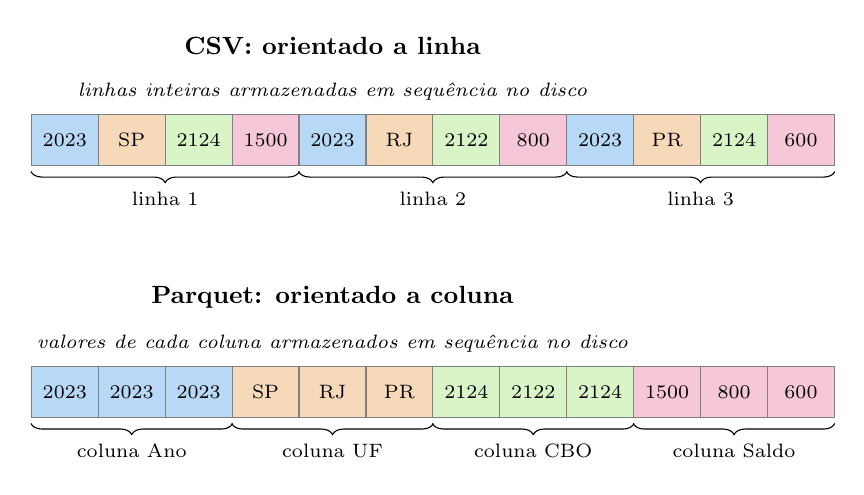
\begin{tikzpicture}[
        every node/.style={font=\footnotesize},
        cell/.style={rectangle, draw=black!50, minimum width=8.5mm, minimum height=6.5mm,
                     inner sep=0pt, font=\scriptsize},
        rotulo/.style={font=\scriptsize\itshape, anchor=north}
    ]
        \definecolor{colAno}{rgb}{0.72, 0.85, 0.96}
        \definecolor{colUF}{rgb}{0.96, 0.85, 0.72}
        \definecolor{colCBO}{rgb}{0.85, 0.96, 0.78}
        \definecolor{colSaldo}{rgb}{0.96, 0.78, 0.85}

        % ===== CSV =====
        \node[font=\small\bfseries] at (0, 3.6) {CSV: orientado a linha};
        \node[rotulo] at (0, 3.25) {linhas inteiras armazenadas em sequência no disco};

        % Linha 1
        \node[cell, fill=colAno]   at (-3.40, 2.4) {2023};
        \node[cell, fill=colUF]    at (-2.55, 2.4) {SP};
        \node[cell, fill=colCBO]   at (-1.70, 2.4) {2124};
        \node[cell, fill=colSaldo] at (-0.85, 2.4) {1500};
        % Linha 2
        \node[cell, fill=colAno]   at ( 0.00, 2.4) {2023};
        \node[cell, fill=colUF]    at ( 0.85, 2.4) {RJ};
        \node[cell, fill=colCBO]   at ( 1.70, 2.4) {2122};
        \node[cell, fill=colSaldo] at ( 2.55, 2.4) {800};
        % Linha 3
        \node[cell, fill=colAno]   at ( 3.40, 2.4) {2023};
        \node[cell, fill=colUF]    at ( 4.25, 2.4) {PR};
        \node[cell, fill=colCBO]   at ( 5.10, 2.4) {2124};
        \node[cell, fill=colSaldo] at ( 5.95, 2.4) {600};

        % Chaves indicando agrupamento por linha
        \draw[decorate, decoration={brace, amplitude=4pt, mirror}]
            (-3.83, 2.0) -- (-0.42, 2.0) node[midway, below=4pt, font=\scriptsize] {linha 1};
        \draw[decorate, decoration={brace, amplitude=4pt, mirror}]
            (-0.43, 2.0) -- (2.98, 2.0)  node[midway, below=4pt, font=\scriptsize] {linha 2};
        \draw[decorate, decoration={brace, amplitude=4pt, mirror}]
            (2.97, 2.0)  -- (6.38, 2.0)  node[midway, below=4pt, font=\scriptsize] {linha 3};

        % ===== PARQUET =====
        \node[font=\small\bfseries] at (0, 0.4) {Parquet: orientado a coluna};
        \node[rotulo] at (0, 0.05) {valores de cada coluna armazenados em sequência no disco};

        % Coluna Ano
        \node[cell, fill=colAno] at (-3.40, -0.8) {2023};
        \node[cell, fill=colAno] at (-2.55, -0.8) {2023};
        \node[cell, fill=colAno] at (-1.70, -0.8) {2023};
        % Coluna UF
        \node[cell, fill=colUF]  at (-0.85, -0.8) {SP};
        \node[cell, fill=colUF]  at ( 0.00, -0.8) {RJ};
        \node[cell, fill=colUF]  at ( 0.85, -0.8) {PR};
        % Coluna CBO
        \node[cell, fill=colCBO] at ( 1.70, -0.8) {2124};
        \node[cell, fill=colCBO] at ( 2.55, -0.8) {2122};
        \node[cell, fill=colCBO] at ( 3.40, -0.8) {2124};
        % Coluna Saldo
        \node[cell, fill=colSaldo] at ( 4.25, -0.8) {1500};
        \node[cell, fill=colSaldo] at ( 5.10, -0.8) {800};
        \node[cell, fill=colSaldo] at ( 5.95, -0.8) {600};

        % Chaves indicando agrupamento por coluna
        \draw[decorate, decoration={brace, amplitude=4pt, mirror}]
            (-3.83, -1.2) -- (-1.27, -1.2) node[midway, below=4pt, font=\scriptsize] {coluna Ano};
        \draw[decorate, decoration={brace, amplitude=4pt, mirror}]
            (-1.28, -1.2) -- (1.28, -1.2)  node[midway, below=4pt, font=\scriptsize] {coluna UF};
        \draw[decorate, decoration={brace, amplitude=4pt, mirror}]
            (1.27, -1.2)  -- (3.83, -1.2)  node[midway, below=4pt, font=\scriptsize] {coluna CBO};
        \draw[decorate, decoration={brace, amplitude=4pt, mirror}]
            (3.82, -1.2)  -- (6.38, -1.2)  node[midway, below=4pt, font=\scriptsize] {coluna Saldo};

    \end{tikzpicture}
    \\[4pt]
    Fonte: Autoria própria.
\end{figure}

No exemplo da \autoref{fig:parquet-vs-csv}, uma consulta como \texttt{SELECT Saldo FROM tabela} obriga o CSV a ler todas as linhas e descartar três quartos dos bytes carregados. No Parquet, a mesma consulta vai direto ao bloco da coluna Saldo e lê apenas o que importa, e esse ganho cresce quando se trabalha com tabelas de dezenas de colunas e milhões de registros, como as deste trabalho.

Essa organização traz três benefícios concretos para consultas analíticas:

\begin{itemize}
    \item \textbf{\textit{Column pruning}}: consultas que selecionam apenas algumas colunas (e.g., \texttt{SELECT uf, SUM(saldo)}) ignoram completamente os blocos de disco das colunas não solicitadas, reduzindo o I/O em proporção ao número de colunas não lidas;

    \item \textbf{\textit{Predicate pushdown}}: filtros numéricos ou de string são avaliados no nível do bloco de dados, usando estatísticas de mínimo e máximo armazenadas nos metadados do arquivo para descartar blocos inteiros sem leitura;

    \item \textbf{Compressão eficiente}: valores de uma mesma coluna tendem a ter distribuição similar, tornando algoritmos de compressão como Snappy e ZSTD mais eficazes do que em formatos orientados a linha. Na prática, converter os arquivos de texto para Parquet com ZSTD reduz substancialmente o espaço em disco; a magnitude exata dessa redução para os microdados da RAIS e do CAGED será quantificada nos resultados deste trabalho. O resultado, ao contrário do texto bruto, passa a ser consultado diretamente por motores OLAP como o DuckDB, sem nenhuma importação prévia.
\end{itemize}

O formato também aceita particionar os arquivos por colunas de alta cardinalidade, como ano e estado \cite{ApacheParquet2024}. Com isso, leitores como o DuckDB conseguem carregar apenas as partições que casam com os filtros da consulta, reforçando o \textit{predicate pushdown} já em nível de arquivo.

\subsection{Motores Analíticos \textit{In-Process}}

Os motores de \textit{Online Analytical Processing} (OLAP) tradicionais, como Redshift, BigQuery ou ClickHouse, seguem o modelo cliente-servidor, o que cobra seu preço em latência de rede e complexidade de operação. Uma alternativa mais recente são os motores \textit{in-process}, executados dentro do próprio processo da aplicação que os usa, sem servidor separado. O DuckDB é o principal representante dessa categoria
\cite{Raasveldt2019}.

Por dentro, o DuckDB usa execução vetorizada (\textit{vectorized execution}): em vez de processar uma linha por vez, como faz um sistema de \textit{Online Transaction Processing} (OLTP), ele opera sobre vetores de valores de uma mesma coluna \cite{Raasveldt2019}. Esse modelo aproveita as instruções de \textit{Single Instruction, Multiple Data} (SIMD) dos processadores modernos e ajuda a maximizar o \textit{throughput} analítico.


\subsection{Armazenamento de Objetos e a API S3}

No armazenamento de objetos (\textit{object storage}), os arquivos são tratados como objetos identificados por uma chave única dentro de um \textit{bucket}, sem a hierarquia rígida de diretórios típica dos sistemas de arquivos tradicionais. Esse modelo casa bem com \textit{data lakes}: escala com facilidade, tolera falhas e suporta acesso paralelo por vários processos ao mesmo tempo \cite{Reis2022}.

O \textit{Amazon Simple Storage Service} (S3) virou a API \textit{de facto} para armazenamento de objetos e é hoje amplamente adotada pelo ecossistema de engenharia de dados. O MinIO é uma implementação de código aberto dessa mesma API, voltada para implantação \textit{on-premises} ou em qualquer nuvem \cite{MinIO2024}. Como segue a S3 à risca, ele funciona sem ajustes com qualquer biblioteca compatível, incluindo o DuckDB (via \texttt{httpfs}), o PyArrow e o Polars \cite{PyArrow2024, Polars2024}.


\section{Visualização de Dados \textit{Web}}

A entrega de análises por meio de \textit{dashboards} interativos na \textit{web} tem sido facilitada pelos \textit{frameworks} de aplicações de dados (\textit{data apps}), que eliminam a barreira entre a análise e a interface: a aplicação é escrita na mesma linguagem em que ocorrem as transformações e os modelos, dispensando uma camada de \textit{front-end} separada. O Streamlit é um exemplo representativo dessa categoria \cite{Streamlit2024}: a cada interação do usuário (filtro, mudança de aba, seleção em um menu), o \textit{script} é reexecutado de cima a baixo, e um sistema de \textit{cache} nativo evita recomputar resultados pesados. Componentes prontos de visualização (gráficos de linha, mapas, tabelas e métricas) e a integração transparente com bibliotecas como Plotly e Altair tornam esse tipo de \textit{framework} conveniente para projetos com camada de dados pesada e interface enxuta.

\section{Modelos de Séries Temporais e \textit{Forecasting}}

Uma série temporal é uma sequência de observações de uma variável ao longo do tempo, coletadas em intervalos regulares \cite{Hyndman2021}. Em análises de mercado de trabalho, costuma-se decompor essa série em quatro componentes: a tendência (o movimento de longo prazo), a sazonalidade (flutuações periódicas e regulares), a ciclicidade (oscilações de médio prazo ligadas a ciclos econômicos) e o ruído (a parte aleatória que sobra depois de identificar os outros três) \cite{Box2015}.

\subsection{Modelos SARIMA}
\label{subsec:sarima}

A família ARIMA (\textit{AutoRegressive Integrated Moving Average}), formalizada por \citeonline{Box2015}, modela uma série a partir de três mecanismos: a dependência da observação atual em relação às anteriores (componente autorregressiva, $p$), a diferenciação necessária para estabilizar o nível da série (componente integrada, $d$) e a dependência em relação aos erros passados (componente de média móvel, $q$). A extensão sazonal, SARIMA, replica esses três mecanismos no período da sazonalidade, e é escrita como
\begin{equation}
    \text{SARIMA}(p, d, q)(P, D, Q)_m,
\end{equation}
em que $(P, D, Q)$ são as ordens sazonais e $m$ é o período --- 12, no caso de séries mensais com ciclo anual.

A diferenciação sazonal ($D = 1$) é o que torna a família adequada à série de saldo de empregos: ela remove o ciclo anual de admissões e desligamentos subtraindo de cada mês o mesmo mês do ano anterior, em lugar de estimar uma forma funcional para esse ciclo. O preço é que a série diferenciada perde os primeiros $m$ pontos, o que importa quando o histórico é curto.

Modelos dessa família pressupõem que o que resta após a modelagem seja ruído sem estrutura. Essa hipótese é verificável: o teste de \citeonline{Ljung1978} examina se as autocorrelações dos resíduos, tomadas em conjunto, diferem do que se esperaria de uma sequência aleatória. Resíduo com estrutura remanescente indica que há sinal que o modelo deixou passar.

A \autoref{fig:serie-decomp} ilustra a decomposição clássica de uma série temporal nos componentes discutidos no início desta seção.

\begin{figure}[htbp]
    \centering
    \caption{Decomposição clássica de uma série temporal}
    \label{fig:serie-decomp}
    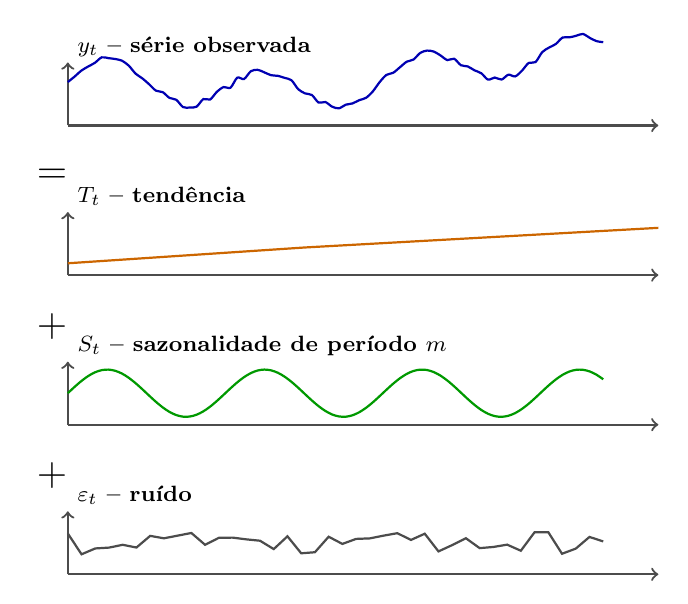
\begin{tikzpicture}[
        every node/.style={font=\scriptsize},
        axe/.style={->, thick, black!70},
        serie/.style={thick, blue!70!black},
        tendencia/.style={thick, orange!80!black},
        sazon/.style={thick, green!60!black},
        ruido/.style={thick, gray!60!black},
        painel/.style={font=\footnotesize\bfseries, anchor=west}
    ]
        % Painel y(t) - serie observada
        \node[painel] at (-4.5, 2.6) {$y_t$ -- série observada};
        \draw[axe] (-4.5, 1.6) -- (-4.5, 2.4);
        \draw[axe] (-4.5, 1.6) -- (3.0, 1.6);
        \draw[serie] plot[smooth, samples=80, domain=0:6.8]
            ({-4.5+\x}, {1.6 + 0.4 + 0.05*\x + 0.25*sin(\x*180) + 0.15*cos(\x*60) + 0.08*rnd});

        % Operador =
        \node[font=\Large] at (-4.7, 0.95) {$=$};

        % Painel tendencia
        \node[painel] at (-4.5, 0.7) {$T_t$ -- tendência};
        \draw[axe] (-4.5, -0.3) -- (-4.5, 0.5);
        \draw[axe] (-4.5, -0.3) -- (3.0, -0.3);
        \draw[tendencia] (-4.5, -0.15) -- (-1.5, 0.05) -- (3.0, 0.30);

        % Operador +
        \node[font=\Large] at (-4.7, -0.95) {$+$};

        % Painel sazonalidade
        \node[painel] at (-4.5, -1.2) {$S_t$ -- sazonalidade de período $m$};
        \draw[axe] (-4.5, -2.2) -- (-4.5, -1.4);
        \draw[axe] (-4.5, -2.2) -- (3.0, -2.2);
        \draw[sazon] plot[smooth, samples=80, domain=0:6.8]
            ({-4.5+\x}, {-1.8 + 0.3*sin(\x*180)});

        % Operador +
        \node[font=\Large] at (-4.7, -2.85) {$+$};

        % Painel ruido
        \node[painel] at (-4.5, -3.1) {$\varepsilon_t$ -- ruído};
        \draw[axe] (-4.5, -4.1) -- (-4.5, -3.3);
        \draw[axe] (-4.5, -4.1) -- (3.0, -4.1);
        \draw[ruido] plot[samples=40, domain=0:6.8]
            ({-4.5+\x}, {-3.7 + 0.15*rand});

    \end{tikzpicture}
    \\[4pt]
    Fonte: Autoria própria, adaptado de \citeonline{Box2015}.
\end{figure}

\subsection{Validação de Origem Móvel}
\label{subsec:origem-movel}

Avaliar um modelo de série temporal por amostragem aleatória é inválido: embaralhar as observações permite ao modelo treinar com o futuro e prever o passado. A alternativa consagrada é a validação de origem móvel \cite{Tashman2000}, também chamada de validação em janelas expansivas: o modelo é treinado com os dados até um instante $T$, prevê os $h$ períodos seguintes, a origem avança e o procedimento se repete. O erro reportado é a média das dobras.

Duas cautelas acompanham o método. A primeira é que o \textit{baseline} de comparação precisa ser avaliado nas mesmas dobras e no mesmo horizonte --- comparar um modelo medido em origem móvel com um \textit{baseline} medido de outra forma não compara nada. A segunda é que uma grade grande de especificações, avaliada em poucas dobras, encontra por acaso o modelo que se sai bem naquelas dobras: é sobreajuste deslocado da amostra de treino para a de validação.

Um \textit{baseline} usual em séries sazonais é o ingênuo sazonal, que prevê para cada mês o valor observado no mesmo mês do ano anterior \cite{Hyndman2021}. Ele é a referência mínima: um modelo que não o supera não se justifica.

\subsection{Métricas de avaliação}
\label{subsec:metricas}

A qualidade das previsões é medida por duas métricas clássicas. O \textit{Mean Absolute Error} (MAE) calcula o erro médio em valores absolutos, na mesma unidade da série. Já o \textit{Root Mean Squared Error} (RMSE) penaliza erros maiores de forma quadrática e, por isso, é mais sensível a previsões que ficam bem longe do valor observado. As duas fórmulas são apresentadas a seguir:

\begin{equation}
    \text{MAE} = \frac{1}{n}\sum_{i=1}^{n}|y_i - \hat{y}_i|
    \qquad
    \text{RMSE} = \sqrt{\frac{1}{n}\sum_{i=1}^{n}(y_i - \hat{y}_i)^2}
\end{equation}

onde $y_i$ é o valor observado e $\hat{y}_i$ é o valor previsto pelo modelo para o período $i$.

\section{Métodos de Decomposição Salarial, Sobrevivência e Agrupamento}

As perguntas sobre qualidade do emprego, equidade e geografia não se respondem com extrapolação de série. Esta seção apresenta os três métodos empregados para elas.

\subsection{Decomposição de Oaxaca-Blinder}
\label{subsec:oaxaca}

Proposta de forma independente por \citeonline{Oaxaca1973} e \citeonline{Blinder1973}, a decomposição separa a diferença média de salários entre dois grupos em duas parcelas. Partindo de uma regressão do logaritmo do salário sobre características produtivas em cada grupo, a diferença das médias se escreve
\begin{equation}
    \bar{Y}_A - \bar{Y}_B =
    \underbrace{(\bar{X}_A - \bar{X}_B)'\beta^{*}}_{\text{explicada}} +
    \underbrace{\bar{X}_A'(\hat{\beta}_A - \beta^{*}) + \bar{X}_B'(\beta^{*} - \hat{\beta}_B)}_{\text{não explicada}},
\end{equation}
em que $\bar{X}$ são as médias das características, $\hat{\beta}$ os coeficientes estimados em cada grupo e $\beta^{*}$ o vetor de referência.

A parcela \textbf{explicada} é a diferença atribuível ao fato de os grupos terem características distintas --- escolaridade, experiência, ocupação, porte da empresa. A parcela \textbf{não explicada} é a diferença que permanece entre pessoas com características equivalentes, isto é, uma diferença de \textit{retorno} às mesmas características.

A escolha de $\beta^{*}$ não é neutra: usar os coeficientes de um dos grupos como referência altera a magnitude das parcelas. \citeonline{Neumark1988} propõe usar os coeficientes da regressão conjunta dos dois grupos, convenção adotada neste trabalho e discutida em detalhe por \citeonline{Jann2008}.

Uma advertência metodológica é essencial: a parcela não explicada \textbf{não é medida de discriminação}. Ela contém tudo que afeta salário e não está no modelo --- experiência anterior não registrada, interrupções de carreira, negociação, preferências por jornada. Ela é um limite superior para o que a discriminação poderia explicar, e não uma estimativa dela.

\subsection{Análise de Sobrevivência e Tábua de Vida de Período}
\label{subsec:sobrevivencia}

A permanência em um emprego é um fenômeno de duração, e o instrumental da análise de sobrevivência se aplica a ele. O estimador de \citeonline{Kaplan1958} é a ferramenta usual quando se acompanha uma coorte ao longo do tempo, tratando como censurados os casos cujo desfecho não foi observado até o fim do acompanhamento.

Há, porém, uma incompatibilidade entre esse estimador e a estrutura da RAIS. A RAIS é um \textbf{corte transversal}: cada edição retrata os vínculos existentes em 31 de dezembro, e não uma coorte seguida no tempo. Em um corte transversal, vínculos longos estão sobre-representados --- quem permanece muitos anos aparece em muitas edições, enquanto quem passou poucos meses pode não aparecer em nenhuma. Aplicar Kaplan-Meier a esse corte produz estimativas de duração infladas.

A alternativa adequada é a \textbf{tábua de vida de período}, instrumento clássico da demografia \cite{Preston2001}. Em vez de seguir uma coorte, ela toma as taxas de saída observadas em cada faixa de duração \textit{em um mesmo ano} e com elas constrói uma sobrevivência sintética: a probabilidade de permanência de uma coorte hipotética que experimentasse, ao longo da vida, as taxas observadas naquele ano. A leitura é diferente e precisa ser declarada --- a tábua descreve o risco vigente no período, não a trajetória de quem entrou em um ano específico.

Complementarmente, um modelo de risco em tempo discreto --- regressão logística da ocorrência do desligamento no ano sobre as características do vínculo --- permite estimar o efeito de cada característica mantendo as demais constantes.

\subsection{Agrupamento por $k$-Médias}
\label{subsec:clusters}

Para descrever a geografia do mercado além de um \textit{ranking} de maiores volumes, é útil agrupar municípios com trajetórias semelhantes. O algoritmo $k$-médias \cite{MacQueen1967} particiona as observações em $k$ grupos minimizando a soma das distâncias quadráticas de cada ponto ao centro do seu grupo.

Duas decisões são necessárias. A primeira é a padronização das variáveis: o algoritmo opera sobre distâncias, e variáveis em escalas distintas dominariam o resultado. A segunda é a escolha de $k$, que o algoritmo não determina. Este trabalho utiliza o coeficiente de silhueta \cite{Rousseeuw1987}, que mede, para cada observação, o quanto ela está mais próxima do próprio grupo do que do grupo vizinho mais próximo, e escolhe o $k$ que maximiza a média desse coeficiente.

\section{Publicação de Dados de Pesquisa}
\label{sec:fair}

Reprodutibilidade em trabalhos de dados exige mais que publicar código: exige que os dados tratados estejam acessíveis. Os princípios FAIR \cite{WilkinsonFair2016} sistematizam esse requisito em quatro atributos --- dados localizáveis, acessíveis, interoperáveis e reutilizáveis.

Repositórios de dados que servem arquivos por HTTP com suporte a requisições parciais (\textit{HTTP range requests}) têm uma propriedade útil para formatos colunares: um motor analítico pode ler o rodapé de metadados do arquivo Parquet, identificar os blocos necessários à consulta e baixar apenas esses trechos, sem transferir o arquivo inteiro. Com isso, um conjunto de dados publicado deixa de ser apenas um arquivo para \textit{download} e passa a ser consultável no lugar onde está \cite{HuggingFaceDatasets2026}.

\section{Trabalhos Relacionados}
\label{sec:relacionados}

A análise quantitativa do mercado de trabalho brasileiro a partir dos microdados da RAIS e do CAGED é tema recorrente em estudos publicados nos últimos anos. \citeonline{SilvaLima2018} lembram que, apesar de cobrir apenas o mercado formal, a RAIS é uma das bases mais ricas para estudar o trabalho no país, justamente pela granularidade e pela longa série histórica que oferece, o que sustenta a escolha das fontes neste trabalho. Esta seção apresenta um recorte de trabalhos que se aproximam, por método ou por objeto, da proposta deste TCC, e termina indicando o que diferencia o presente trabalho dos demais.

O Instituto de Pesquisa Econômica Aplicada (IPEA) mantém uma série regular de relatórios de \textit{Conjuntura do Mercado de Trabalho no Brasil}, com edições trimestrais que cruzam dados da Pesquisa Nacional por Amostra de Domicílios Contínua (PNAD Contínua), do CAGED e da RAIS \cite{IPEA2023}. Esses relatórios oferecem uma fotografia agregada do mercado nacional, mas seu foco é macroeconômico: discutem população ocupada, taxa de desemprego e rendimento médio em recortes amplos, sem se aprofundar em um setor específico como TI.

A pesquisa da FECOMERCIOSP, baseada em microdados da RAIS entre 2012 e 2022, analisou 30 ocupações ligadas à tecnologia e quantificou o crescimento do setor em até 95\% no período, com famílias específicas chegando a 740\% \cite{Fecomercio2024}. Esse estudo é o que mais se aproxima da proposta deste TCC, mas se limita à análise descritiva de séries históricas anuais, sem aplicar modelagem preditiva nem integrar o CAGED ao recorte. Além disso, o estudo é publicado como nota técnica, sem detalhamento metodológico que permita a reprodução dos resultados.

A BRASSCOM publica anualmente seu \textit{Relatório Setorial do Macrossetor TIC}, que combina dados da RAIS, CAGED e outras fontes para estimar o tamanho do setor, sua participação no PIB e o déficit projetado de profissionais \cite{Brasscom2024, Brasscom2025}. O recorte do trabalho é setorial e bastante completo, mas a metodologia e os dados intermediários não são abertos: a publicação traz números agregados, sem disponibilizar os \textit{pipelines} ou as bases tratadas que os geraram.

No campo técnico, a Arquitetura Medalhão proposta originalmente pela Databricks \cite{MicrosoftMedallion2024} tornou-se referência para organização de \textit{data lakes}, sendo adotada em estudos de caso e em projetos corporativos para a estruturação de dados em camadas progressivas de qualidade. Em uma direção complementar, \citeonline{Armbrust2021} introduziram o conceito de \textit{lakehouse}, uma evolução do \textit{data lake} que combina o desempenho analítico de \textit{data warehouses} tradicionais com a flexibilidade de armazenamento de dados brutos sobre formatos abertos como Parquet. A proposta defende que motores analíticos modernos, lendo direto sobre arquivos colunares em armazenamento de objetos, podem entregar latência competitiva sem a complexidade operacional de ambientes proprietários, a mesma intuição que motiva as escolhas técnicas deste trabalho. Ainda assim, a aplicação dessa arquitetura especificamente a microdados governamentais brasileiros, com motores leves como o DuckDB e armazenamento S3-compatível, é pouco documentada em trabalhos acadêmicos publicados.

A \autoref{tab:comparativo-relacionados} resume como este TCC se posiciona frente a esses trabalhos, comparando as fontes de dados, o período coberto, o recorte setorial, o uso de modelagem preditiva e a reprodutibilidade.

\begin{table}[htbp]
    \centering
    \caption{Comparação entre os trabalhos relacionados e a proposta deste TCC}
    \label{tab:comparativo-relacionados}
    \footnotesize
    \renewcommand{\arraystretch}{1.35}
    \begin{tabularx}{\textwidth}{%
        >{\raggedright\arraybackslash\hsize=1.20\hsize}X
        >{\raggedright\arraybackslash\hsize=1.00\hsize}X
        >{\raggedright\arraybackslash\hsize=0.90\hsize}X
        >{\raggedright\arraybackslash\hsize=1.10\hsize}X
        >{\raggedright\arraybackslash\hsize=1.00\hsize}X
        >{\raggedright\arraybackslash\hsize=0.80\hsize}X}
        \toprule
        \rowcolor{black!8}
        \textbf{Trabalho} & \textbf{Fontes} & \textbf{Período} & \textbf{Recorte} & \textbf{Modelagem preditiva} & \textbf{Reprodu\-tível} \\
        \midrule
        IPEA            & PNAD Contínua, CAGED, RAIS  & Até 2023 (trimestral) & Macroeconômico (todo o mercado) & Não & Não \\
        FECOMERCIOSP & RAIS                     & 2012--2022 & TI (30 ocupações) & Não & Não \\
        BRASSCOM & RAIS, CAGED e outras & Anual & Macrossetor TIC & Projeção de déficit & Não (dados fechados) \\
        \rowcolor{blue!6}
        \textbf{Este TCC}               & RAIS + CAGED integradas & 2007--2026 (mensal/anual) & TI por CBO, CNAE e UF & SARIMA validado em origem móvel e \textit{nowcast} do estoque & Sim (código e dados abertos) \\
        \bottomrule
    \end{tabularx}
    \\[4pt]
    Fonte: Autoria própria.
\end{table}

Esses trabalhos, em conjunto, deixam três lacunas que este TCC pretende preencher. A primeira é a integração das duas bases (RAIS e CAGED) em uma série única e harmonizada, cobrindo dezoito anos de dados. A segunda é a aplicação de modelos formais --- previsão da série mensal com especificação escolhida por validação de origem móvel e estimação do estoque corrente por \textit{nowcast} ---, o que vai além da análise descritiva. A terceira é a oferta de uma plataforma analítica reprodutível, em que tanto o \textit{pipeline} quanto o \textit{dashboard} podem ser inspecionados, executados e estendidos por outros pesquisadores.

Os conceitos apresentados neste capítulo dão a base para entender as escolhas técnicas e metodológicas descritas no \autoref{cap:metodologia}.
